%%\documentclass{beamer}
%%\documentclass[handout,usenames,dvipsnames]{beamer}
\documentclass[usenames,dvipsnames]{beamer}
\usepackage[numbers,totalnumber,sidebarshades]{beamerthemeUppsala}

\usepackage[utf8]{inputenc}
\usepackage[T1]{fontenc}
\usepackage{xcolor}
\usepackage{import}
\usepackage{listings}
\usepackage{hyperref}

%%%%%% Bibliograpy as footnotes %%%%
\usepackage{graphicx}
\usepackage[giveninits=true]{biblatex}
%\bibliography{../1DL010-21}

\graphicspath{{imgs/}}

\usepackage{pgfpages}
%\setbeameroption{show notes on second screen}
\setbeamertemplate{note page}{\insertnote}

%%\setbeamercovered{transparent}

\usepackage{xspace}
\usepackage{stmaryrd}
\usepackage{comment}

\newcommand{\tc}{\textcolor}
\newcommand{\largeskip}{\vspace{1cm}}
\newcommand{\nat}{\ensuremath{\mathbb{N}}}
\newcommand{\ra}{\ensuremath{\rightarrow}}

\newcommand{\states}{\ensuremath{S}}
\newcommand{\sts}{\ensuremath{s}}
\newcommand{\inits}{\ensuremath{s_I}}
\newcommand{\isg}{\ensuremath{g}}
\newcommand{\actions}{\ensuremath{A}}
\newcommand{\actf}{\ensuremath{\mathsf{av}}}
\newcommand{\acta}{\ensuremath{a}}
\newcommand{\trf}{\ensuremath{\delta}}
\newcommand{\costf}{\ensuremath{c}}
\newcommand{\utilf}{\ensuremath{u}}

\newcommand{\players}{\ensuremath{P}}
\newcommand{\maxp}{\ensuremath{\text{\textsc{max}}}}
\newcommand{\minp}{\ensuremath{\text{\textsc{min}}}}

\newcommand{\pts}{\ensuremath{PTS}}
\newcommand{\gts}{\ensuremath{GTS}}

\newcommand{\bstates}{\ensuremath{Q}}
\newcommand{\stb}{\ensuremath{q}}
\newcommand{\isf}{\ensuremath{f}}

\newcommand{\set}[1]{\ensuremath{ \{ #1 \}}}
\newcommand{\ol}{\ensuremath{\overline}}

\newcommand{\turnf}{\ensuremath{t}}

%%\newcommand{\land}{\wedge}
%%\newcommand{\lor}{\wee}
\newcommand{\lra}{\leftrightarrow}
\newcommand{\propl}{\mathcal{L}_p}

\newcommand{\M}{\mathcal{M}}
\newcommand{\lang}{\mathcal{L}}
\newcommand{\sat}{\ensuremath{\mathsf{SAT}}\xspace}
\newcommand{\limp}{\ensuremath{\mathsf{LIMP}}\xspace}

\newcommand{\const}{\boldsymbol}
\newcommand{\terms}{\mathit{TM}}
\newcommand{\term}{t}
\newcommand{\atoms}{ATOM}
\newcommand{\forms}{FORM}
\newcommand{\fv}{FV}
\newcommand{\struct}{\mathcal{S}}
\newcommand{\dom}{\Delta}

\newcommand{\intf}{I}

\newcommand{\te}{\ensuremath{\bar{v}}}
\newcommand{\va}{\ensuremath{v}}

\newcommand{\quant}{\ensuremath{\mathcal{Q}}}

\newcommand{\reals}{\ensuremath{\mathbb{R}}}

\newcommand{\hsig}{\ensuremath{h_{sig}}}
\newcommand{\logl}{\ensuremath{L_{\ell \ell}}}

\newcommand{\vechsig}{\ensuremath{\bar{h}_{sig}}}


%%%%%%%%%%%% Fabio ML %%%%%%%%%%%%%%%%%%
\def\riga{\vskip 1\baselineskip \noindent}
\newcommand{\bi}{\begin{itemize}\setlength{\itemsep}{-0.1em}}
\newcommand{\ei}{\end{itemize}}
\newcommand{\be}{\begin{enumerate}}
\newcommand{\ee}{\end{enumerate}}
%%%%%%%%%%%%%%%%%%%%%%%%%%%%%%%%%%%



%%%%%%%%%%% FNN %%%%%%%%%%%%%%%%%%%%
\newcommand{\nnw}[2]{w^{(#1)}_{#2}}
\newcommand{\nnW}[1]{\pmb{W}^{(#1)}}
\newcommand{\nna}[2]{a^{(#1)}_{#2}}
\newcommand{\nnA}[1]{\pmb{a}^{(#1)}}
\newcommand{\nnz}[2]{z^{(#1)}_{#2}}
\newcommand{\nnZ}[1]{\pmb{z}^{(#1)}}
\newcommand{\nnh}{\pmb{h}}
\newcommand{\nndelta}[2]{\delta^{(#1)}_{#2}}
\newcommand{\nnDELTA}[2]{\Delta^{(#1)}_{#2}}
\newcommand{\nnDelta}[1]{\pmb{\delta}^{(#1)}}
\newcommand{\nnDDELTA}[1]{\pmb{\Delta}^{(#1)}}


%%%%%%%%%%%%%%%%%%%%%%%%%%%%%%%%%%






\newcommand{\norm}[1]{\left\lVert#1\right\rVert}
%%%%%%%%%%%%%%%%%%%%%%%%%%%%%%%%%%%%%%%%
\title{1DT109 - Accelerating systems with FPGAs}
\subtitle{Unstable gradients}

\author[R.\ De Masellis]{Riccardo De Masellis}
\date[]{\today}
\institute[uu.se]{Uppsala University}

\begin{document}

\begin{frame}[plain]
  \titlepage
\end{frame}
%%%%%%%%%%%%%%%%%%%%%%%%%%%%%%%%%%%%%%%
%\section{Universality of Neural Networks}
%\frame{
%\setbeamercovered{transparent}
%\tableofcontents[currentsection,
%        currentsubsection,
%        subsectionstyle=shaded]
%}
%%%%%%%%%%%%%%%%%%%%%%%%%%%%%%%%%%%%%%%
\begin{frame}
   \frametitle{Recap}
   
   Universality theorem says that one hidden layer is enough to approximate any continuous function. However:
  
  \vfill
  
  \begin{ntblock}
  \centering
  In many tasks, e.g., visual pattern recognition \\ deep networks are a better choice.
  \end{ntblock}
  
  \vfill
  
  \flushleft
Sometimes having multiple layers reduces the number of total neurons\footnote{Something similar happens with circuits depth as well.}.
  
\end{frame}

%%%%%%%%%%%%%%%%%%%%%%%%%%%%%%%%%%%%%%%
\begin{frame}
\frametitle{How do we train deep networks?}

\begin{alertblock}{Problem}
\centering
Layers learn at different speeds. In particular, early layers barely change their weights at all (but it could happen the other way around as well).	
\end{alertblock}

\end{frame}
%%%%%%%%%%%%%%%%%%%%%%%%%%%%%%%%%%%%%%%
\begin{frame}
\frametitle{The vanishing gradient problem}

\begin{minipage}[c]{.45\textwidth}
	\centering
	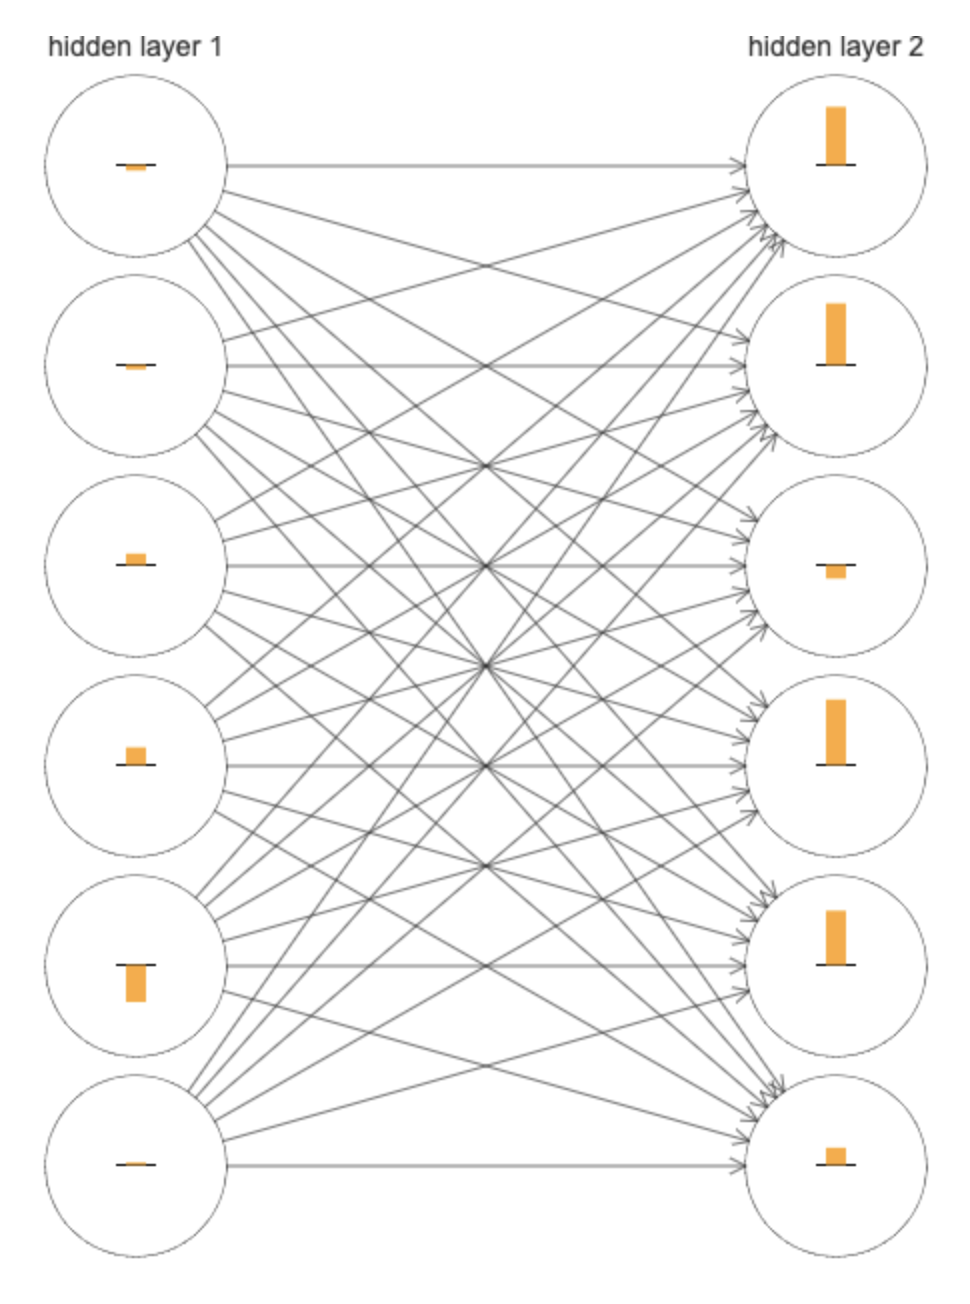
\includegraphics[scale=.3]{learn-speed} 
\end{minipage} \hfill \begin{minipage}[c]{.45\textwidth}
Network $[748, 30, 30, 10]$, showing only the top six neurons of the two hidden layers.


Bars represent $\frac{\partial C}{\partial b}$ for each neuron, on the MNIST digits, at the beginning of the training.
\end{minipage}

  
\end{frame}

%%%%%%%%%%%%%%%%%%%%%%%%%%%%%%%%%%%%%%%
\begin{frame}
\frametitle{Coincidence? Don't think so...}

\begin{itemize}
  \item $\delta^\ell_j = \frac{\partial C}{\partial b^\ell_j}$, ``gradient''\footnote{not really, only for the bias} of $j$-th neuron in $\ell$-th layer;
  \item $\delta^\ell$ vector of all ``gradients'' of the $\ell$-th layer;
  \item with $\norm{\delta^\ell} = \sqrt[2]{\delta^\ell_1 + \ldots + \delta^\ell_n}$, with $n$ number of neuron in layer $\ell$, we denote the ``speed'' of learning of layer $\ell$.
\end{itemize}

\vfill \pause

On the example above we get:
\begin{itemize}
  \item $\norm{\delta^1} = 0.07$
  \item $\norm{\delta^2} = 0.31$
\end{itemize}

\vfill \pause
With a $[784, 30, 30, 30, 10]$ we get:
\begin{itemize}
  \item $\norm{\delta^1} = 0.012$
  \item $\norm{\delta^2} = 0.060$
  \item $\norm{\delta^3} = 0.283$
\end{itemize}

  
\end{frame}


%%%%%%%%%%%%%%%%%%%%%%%%%%%%%%%%%%%%%%%
\begin{frame}
\frametitle{Does training change things?}

Batch gradient descent, 1000 images, 500 epochs.

\centering
	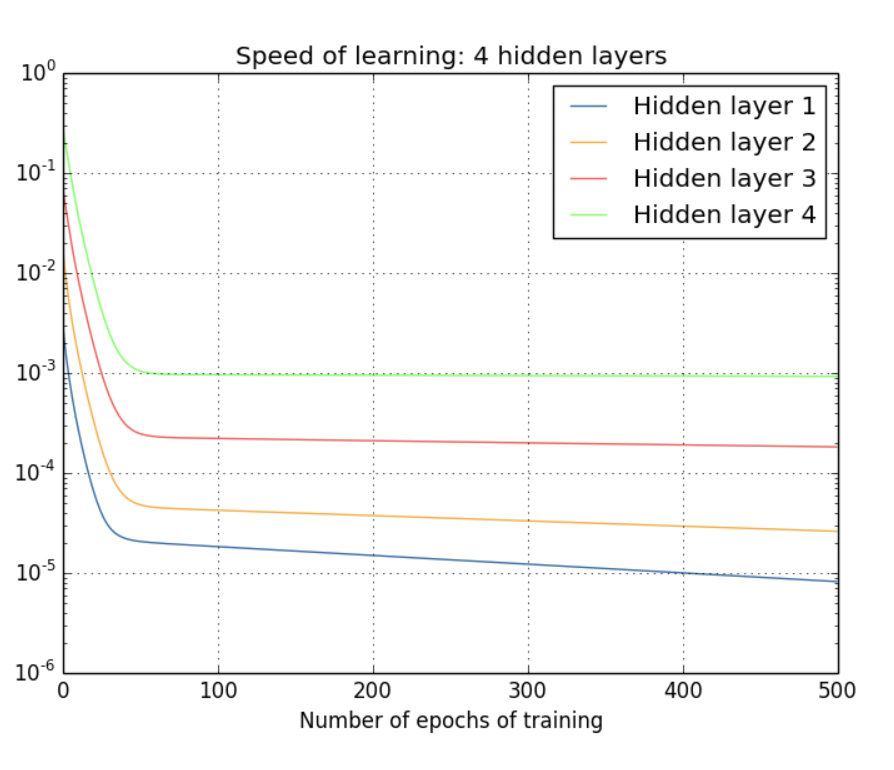
\includegraphics[scale=.3]{speed-graph}
	
\flushleft
\begin{itemize}
  \item The speed of learning start slower in earlier layers;
  \item it keeps being slower during the training (100 ratio).
\end{itemize}
	
\end{frame}

%%%%%%%%%%%%%%%%%%%%%%%%%%%%%%%
%%%%%%%%%%%%%%%%%%%
\begin{frame}
  \frametitle{Let's analyse a simple network...}
  
  \centering
  	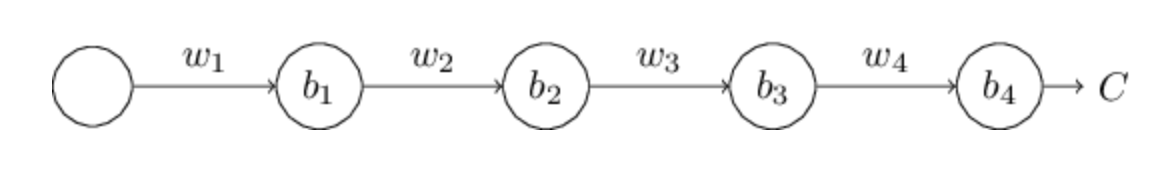
\includegraphics[scale=.3]{simple-net}
  	
  	\flushleft
  	Let's analyse $\frac{\partial C}{\partial b_1}$:
  	
  \centering
    	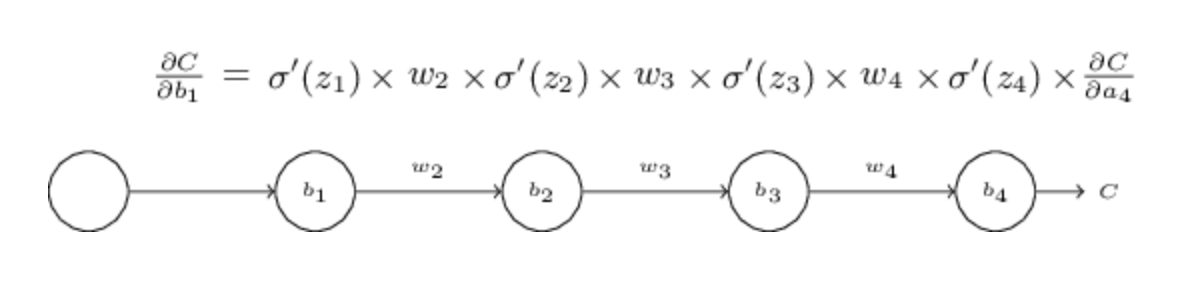
\includegraphics[scale=.5]{deriv-chain}
    	
    	\flushleft
  \begin{itemize}
  \item $a_j = \sigma(z_{j})$
  \item $z_j = w_j a_{j-1} + b_j$
\end{itemize}

  
\end{frame}
%%%%%%%%%%%%%%%%%%%%%%%%%%%%%%%%%%%%%%%%%%%%%
\begin{frame}
  \frametitle{...carefully!}
  
\begin{minipage}[c]{.45\textwidth}
	\centering
	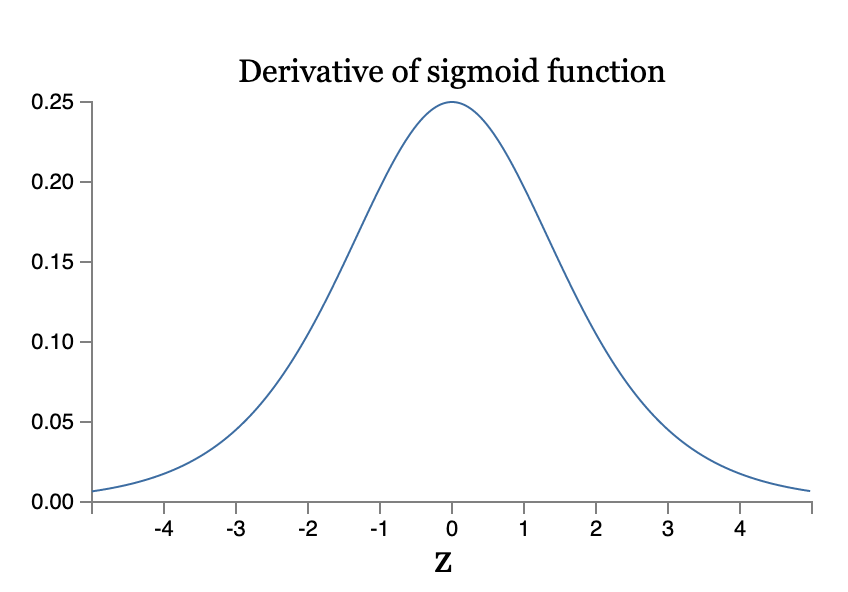
\includegraphics[scale=.4]{sigma-deriv} 
\end{minipage} \hfill \begin{minipage}[c]{.45\textwidth}
\begin{itemize}
  \item Maximum is at $\sigma'(0) = \frac{1}{4}$;
  \item $|w_j| < 1$ because they are initialised according to a Gaussian with mean $0$ and standard deviation $1$.
 \end{itemize}
\end{minipage}

\centering \pause

\[ |w_j \sigma'(z_j) | < \frac{1}{4} \]


\begin{alertblock}{Vanishing gradient explained!}
The more such terms are multiplied, 	the smallest the product becomes.
\end{alertblock}
\end{frame}

%%%%%%%%%%%%%%%%%%%%%%%%%%%%%%%%%%%%%%%%%%%%%
\begin{frame}
  \frametitle{The exploding gradient}
  
  If, during the learning, it happens that terms $|w_j \sigma'(z_j)|$ are (much) larger than $1$, then multiplied together we get an exploding gradient.
  
  \largeskip
  
  \begin{ntblock}
  \centering
  However, this does not happen often in practice.	
  \end{ntblock}
\end{frame}

%%%%%%%%%%%%%%%%%%%%%%%%%%%%%%%%%%%%%%%%%

\begin{frame}
\frametitle{How to cope with unstable gradient}

Again, it's kind of heuristic:

\begin{itemize}
  \item For image recognition, using convolutional neural network helps;
  \item using rectified linear activation functions \emph{usually} speeds up the training;
  \item initialise the weights to neurons as Gaussian random variables with mean $0$ and standard deviation $\frac{1}{\sqrt{n_{in}}}$ where $n_{in}$ is the number of inputs of the neuron.
\end{itemize}


	
\end{frame}








%%%%%%%%%%%%%
%%%%%%%%%%%%%%%%%%%%%%%%%%%%%%%%



%%%%%%%%%%%%%%%%%%%%%%%%%%%%%%%%%%%%%%%%%
\end{document}